\begin{figure}[h]
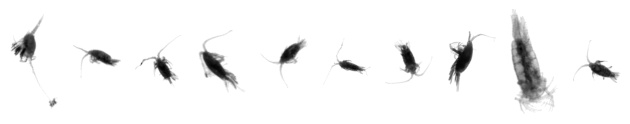
\includegraphics[width=\columnwidth]{collage/000_Candaciidae.jpg}\caption{Samples from the class Candaciidae }
\end{figure}
\begin{figure}[h]
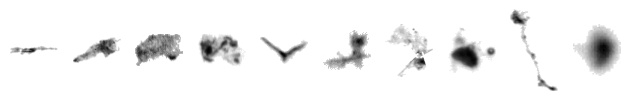
\includegraphics[width=\columnwidth]{collage/001_detritus.jpg}\caption{Samples from the class detritus }
\end{figure}
\begin{figure}[h]
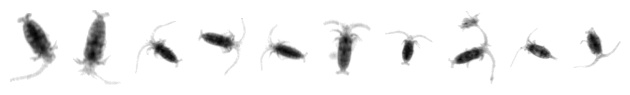
\includegraphics[width=\columnwidth]{collage/002_Calocalanus_pavo.jpg}\caption{Samples from the class Calocalanus pavo }
\end{figure}
\begin{figure}[h]
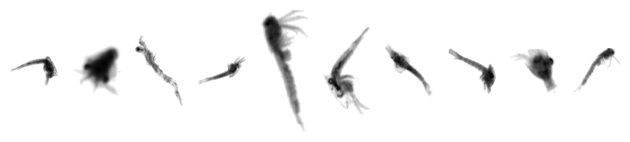
\includegraphics[width=\columnwidth]{collage/003_larvae__Crustacea.jpg}\caption{Samples from the class larvae  Crustacea }
\end{figure}
\begin{figure}[h]
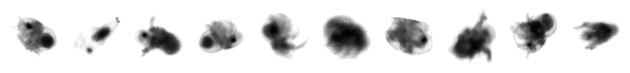
\includegraphics[width=\columnwidth]{collage/004_Podon.jpg}\caption{Samples from the class Podon }
\end{figure}
\begin{figure}[h]
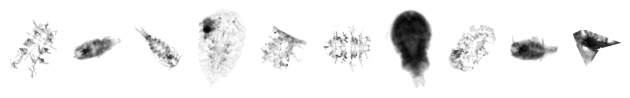
\includegraphics[width=\columnwidth]{collage/005_Sapphirinidae.jpg}\caption{Samples from the class Sapphirinidae }
\end{figure}
\begin{figure}[h]
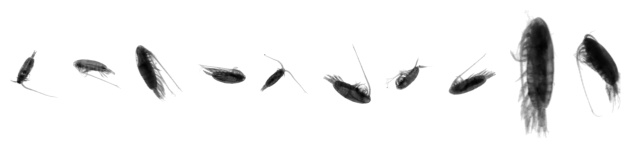
\includegraphics[width=\columnwidth]{collage/006_Calanidae.jpg}\caption{Samples from the class Calanidae }
\end{figure}
\begin{figure}[h]
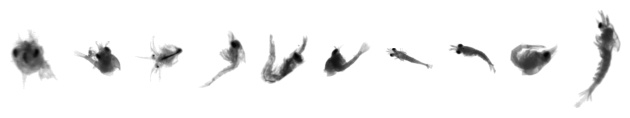
\includegraphics[width=\columnwidth]{collage/007_zoea__Decapoda.jpg}\caption{Samples from the class zoea  Decapoda }
\end{figure}
\begin{figure}[h]
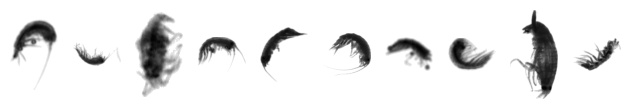
\includegraphics[width=\columnwidth]{collage/008_Gammaridea.jpg}\caption{Samples from the class Gammaridea }
\end{figure}
\begin{figure}[h]
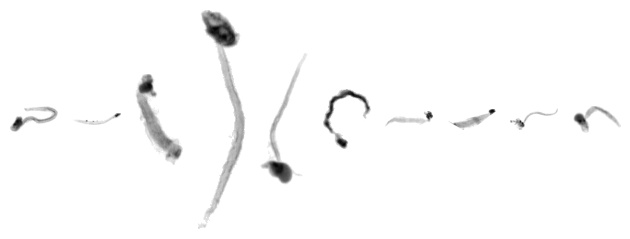
\includegraphics[width=\columnwidth]{collage/009_Oikopleuridae.jpg}\caption{Samples from the class Oikopleuridae }
\end{figure}
\begin{figure}[h]
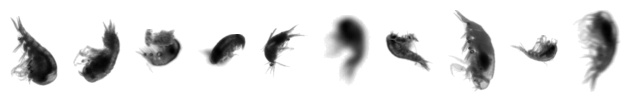
\includegraphics[width=\columnwidth]{collage/010_Hyperiidea.jpg}\caption{Samples from the class Hyperiidea }
\end{figure}
\begin{figure}[h]
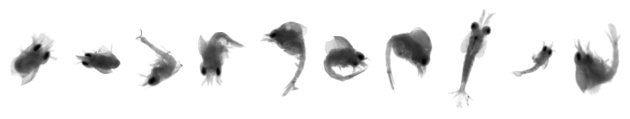
\includegraphics[width=\columnwidth]{collage/011_zoea__Galatheidae.jpg}\caption{Samples from the class zoea  Galatheidae }
\end{figure}
\begin{figure}[h]
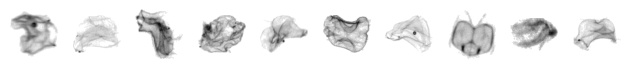
\includegraphics[width=\columnwidth]{collage/012_nectophore__Physonectae.jpg}\caption{Samples from the class nectophore  Physonectae }
\end{figure}
\begin{figure}[h]
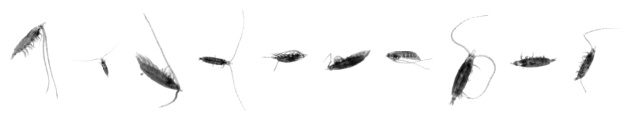
\includegraphics[width=\columnwidth]{collage/013_Rhincalanidae.jpg}\caption{Samples from the class Rhincalanidae }
\end{figure}
\begin{figure}[h]
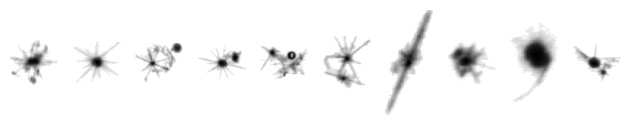
\includegraphics[width=\columnwidth]{collage/014_Acantharea.jpg}\caption{Samples from the class Acantharea }
\end{figure}
\begin{figure}[h]
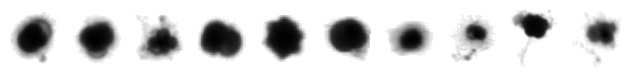
\includegraphics[width=\columnwidth]{collage/015_Foraminifera.jpg}\caption{Samples from the class Foraminifera }
\end{figure}
\begin{figure}[h]
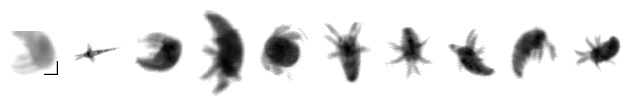
\includegraphics[width=\columnwidth]{collage/016_nauplii__Crustacea.jpg}\caption{Samples from the class nauplii  Crustacea }
\end{figure}
\begin{figure}[h]
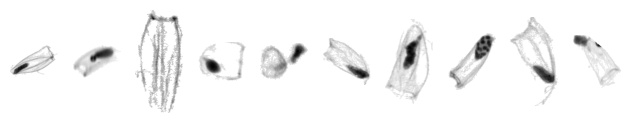
\includegraphics[width=\columnwidth]{collage/017_gonophore__Diphyidae.jpg}\caption{Samples from the class gonophore  Diphyidae }
\end{figure}
\begin{figure}[h]
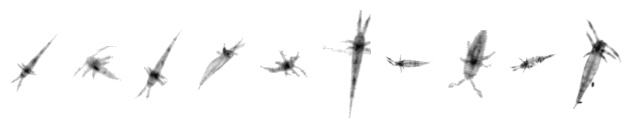
\includegraphics[width=\columnwidth]{collage/018_metanauplii.jpg}\caption{Samples from the class metanauplii }
\end{figure}
\begin{figure}[h]
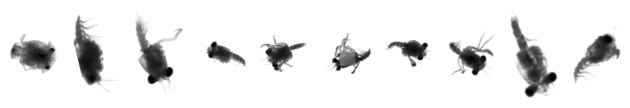
\includegraphics[width=\columnwidth]{collage/019_megalopa.jpg}\caption{Samples from the class megalopa }
\end{figure}
\begin{figure}[h]
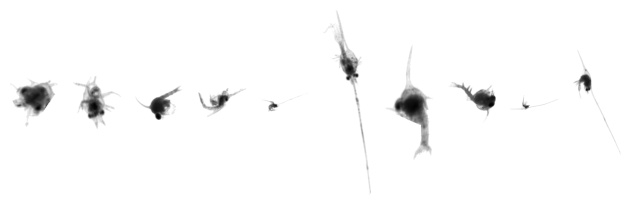
\includegraphics[width=\columnwidth]{collage/020_Brachyura.jpg}\caption{Samples from the class Brachyura }
\end{figure}
\begin{figure}[h]
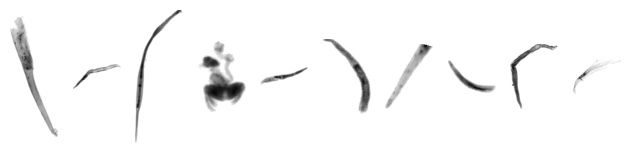
\includegraphics[width=\columnwidth]{collage/021_tail__Chaetognatha.jpg}\caption{Samples from the class tail  Chaetognatha }
\end{figure}
\begin{figure}[h]
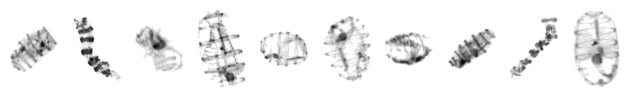
\includegraphics[width=\columnwidth]{collage/022_Doliolida.jpg}\caption{Samples from the class Doliolida }
\end{figure}
\begin{figure}[h]
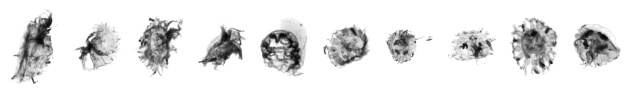
\includegraphics[width=\columnwidth]{collage/023_Scyphozoa.jpg}\caption{Samples from the class Scyphozoa }
\end{figure}
\begin{figure}[h]
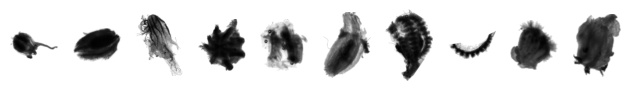
\includegraphics[width=\columnwidth]{collage/024_Ctenophora.jpg}\caption{Samples from the class Ctenophora }
\end{figure}
\begin{figure}[h]
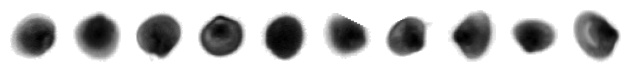
\includegraphics[width=\columnwidth]{collage/025_Bivalvia__Mollusca.jpg}\caption{Samples from the class Bivalvia  Mollusca }
\end{figure}
\begin{figure}[h]
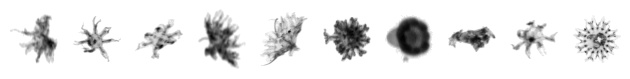
\includegraphics[width=\columnwidth]{collage/026_ephyra.jpg}\caption{Samples from the class ephyra }
\end{figure}
\begin{figure}[h]
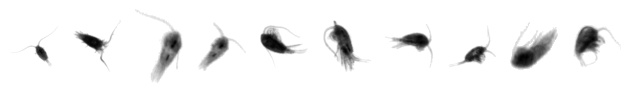
\includegraphics[width=\columnwidth]{collage/027_Temoridae.jpg}\caption{Samples from the class Temoridae }
\end{figure}
\begin{figure}[h]
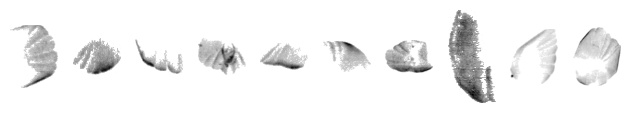
\includegraphics[width=\columnwidth]{collage/028_scale.jpg}\caption{Samples from the class scale }
\end{figure}
\begin{figure}[h]
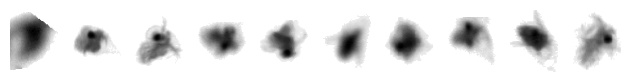
\includegraphics[width=\columnwidth]{collage/029_Evadne.jpg}\caption{Samples from the class Evadne }
\end{figure}
\begin{figure}[h]
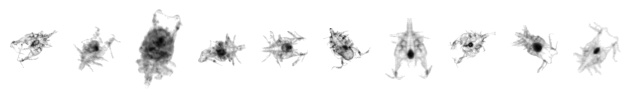
\includegraphics[width=\columnwidth]{collage/030_Copilia.jpg}\caption{Samples from the class Copilia }
\end{figure}
\begin{figure}[h]
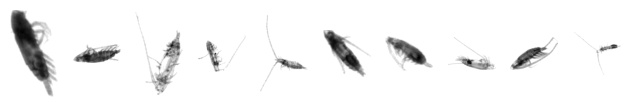
\includegraphics[width=\columnwidth]{collage/031_Eucalanidae.jpg}\caption{Samples from the class Eucalanidae }
\end{figure}
\begin{figure}[h]
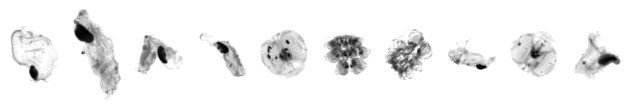
\includegraphics[width=\columnwidth]{collage/032_Pyrosomatida.jpg}\caption{Samples from the class Pyrosomatida }
\end{figure}
\begin{figure}[h]
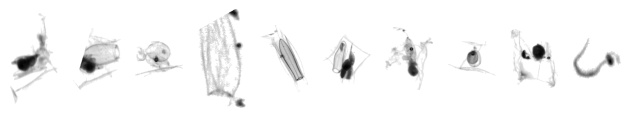
\includegraphics[width=\columnwidth]{collage/033_nectophore__Abylopsis_tetragona.jpg}\caption{Samples from the class nectophore  Abylopsis tetragona }
\end{figure}
\begin{figure}[h]
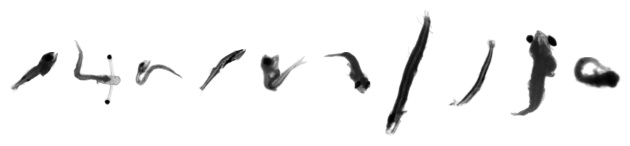
\includegraphics[width=\columnwidth]{collage/034_Actinopterygii.jpg}\caption{Samples from the class Actinopterygii }
\end{figure}
\begin{figure}[h]
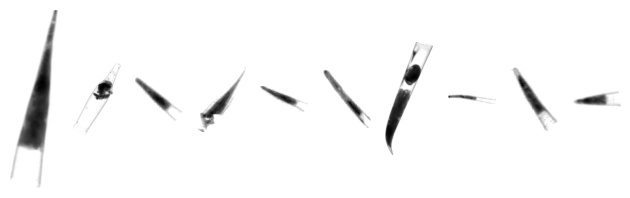
\includegraphics[width=\columnwidth]{collage/035_Creseidae.jpg}\caption{Samples from the class Creseidae }
\end{figure}
\begin{figure}[h]
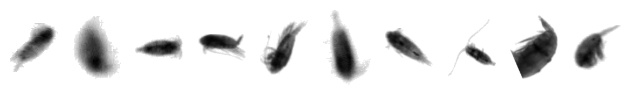
\includegraphics[width=\columnwidth]{collage/036_Calanoida.jpg}\caption{Samples from the class Calanoida }
\end{figure}
\begin{figure}[h]
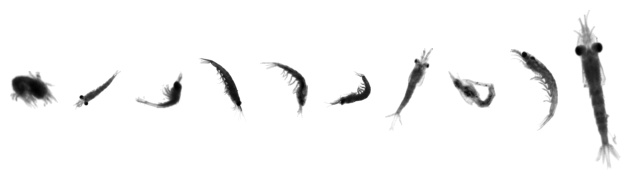
\includegraphics[width=\columnwidth]{collage/037_Decapoda.jpg}\caption{Samples from the class Decapoda }
\end{figure}
\begin{figure}[h]
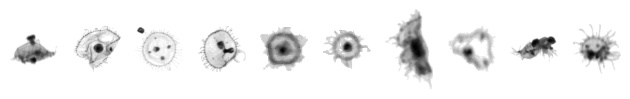
\includegraphics[width=\columnwidth]{collage/038_Obelia.jpg}\caption{Samples from the class Obelia }
\end{figure}
\begin{figure}[h]
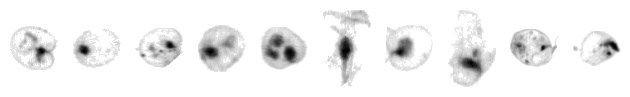
\includegraphics[width=\columnwidth]{collage/039_Noctiluca.jpg}\caption{Samples from the class Noctiluca }
\end{figure}
\begin{figure}[h]
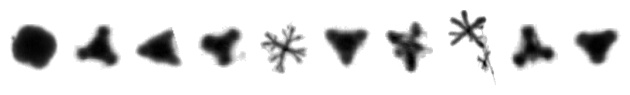
\includegraphics[width=\columnwidth]{collage/040_Spumellaria.jpg}\caption{Samples from the class Spumellaria }
\end{figure}
\begin{figure}[h]
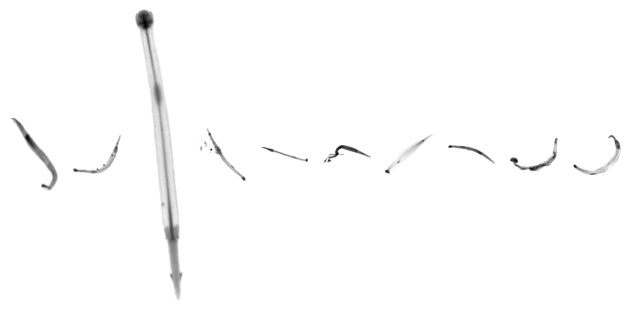
\includegraphics[width=\columnwidth]{collage/041_Chaetognatha.jpg}\caption{Samples from the class Chaetognatha }
\end{figure}
\begin{figure}[h]
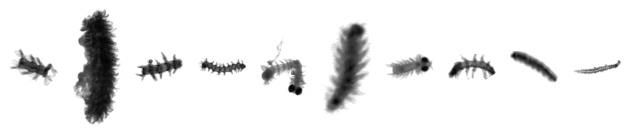
\includegraphics[width=\columnwidth]{collage/042_Annelida.jpg}\caption{Samples from the class Annelida }
\end{figure}
\begin{figure}[h]
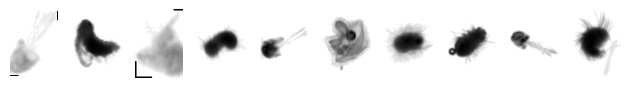
\includegraphics[width=\columnwidth]{collage/043_larvae__Annelida.jpg}\caption{Samples from the class larvae  Annelida }
\end{figure}
\begin{figure}[h]
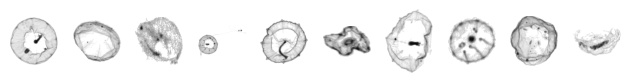
\includegraphics[width=\columnwidth]{collage/044_Rhopalonema.jpg}\caption{Samples from the class Rhopalonema }
\end{figure}
\begin{figure}[h]
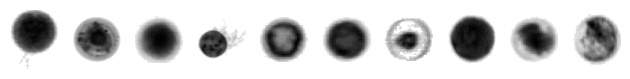
\includegraphics[width=\columnwidth]{collage/045_egg__other.jpg}\caption{Samples from the class egg  other }
\end{figure}
\begin{figure}[h]
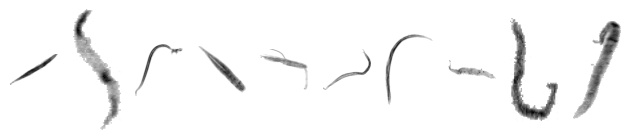
\includegraphics[width=\columnwidth]{collage/046_tail__Appendicularia.jpg}\caption{Samples from the class tail  Appendicularia }
\end{figure}
\begin{figure}[h]
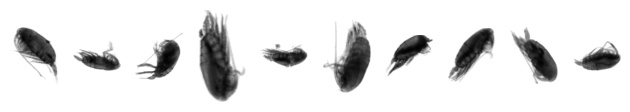
\includegraphics[width=\columnwidth]{collage/047_Euchirella.jpg}\caption{Samples from the class Euchirella }
\end{figure}
\begin{figure}[h]
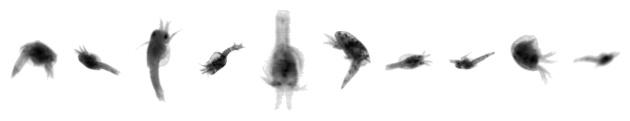
\includegraphics[width=\columnwidth]{collage/048_calyptopsis.jpg}\caption{Samples from the class calyptopsis }
\end{figure}
\begin{figure}[h]
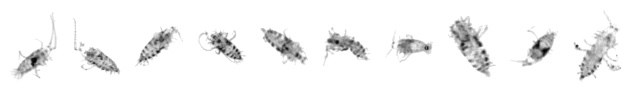
\includegraphics[width=\columnwidth]{collage/049_Haloptilus.jpg}\caption{Samples from the class Haloptilus }
\end{figure}
\begin{figure}[h]
\includegraphics[width=\columnwidth]{collage/050_eudoxie__Diphyidae.jpg}\caption{Samples from the class eudoxie  Diphyidae }
\end{figure}
\begin{figure}[h]
\includegraphics[width=\columnwidth]{collage/051_egg__Actinopterygii.jpg}\caption{Samples from the class egg  Actinopterygii }
\end{figure}
\begin{figure}[h]
\includegraphics[width=\columnwidth]{collage/052_nectophore__Diphyidae.jpg}\caption{Samples from the class nectophore  Diphyidae }
\end{figure}
\begin{figure}[h]
\includegraphics[width=\columnwidth]{collage/053_head.jpg}\caption{Samples from the class head }
\end{figure}
\begin{figure}[h]
\includegraphics[width=\columnwidth]{collage/054_Penilia.jpg}\caption{Samples from the class Penilia }
\end{figure}
\begin{figure}[h]
\includegraphics[width=\columnwidth]{collage/055_egg__Cavolinia_inflexa.jpg}\caption{Samples from the class egg  Cavolinia inflexa }
\end{figure}
\begin{figure}[h]
\includegraphics[width=\columnwidth]{collage/056_Pontellidae.jpg}\caption{Samples from the class Pontellidae }
\end{figure}
\begin{figure}[h]
\includegraphics[width=\columnwidth]{collage/057_Coscinodiscus.jpg}\caption{Samples from the class Coscinodiscus }
\end{figure}
\begin{figure}[h]
\includegraphics[width=\columnwidth]{collage/058_Acartiidae.jpg}\caption{Samples from the class Acartiidae }
\end{figure}
\begin{figure}[h]
\includegraphics[width=\columnwidth]{collage/059_Corycaeidae.jpg}\caption{Samples from the class Corycaeidae }
\end{figure}
\begin{figure}[h]
\includegraphics[width=\columnwidth]{collage/060_artefact.jpg}\caption{Samples from the class artefact }
\end{figure}
\begin{figure}[h]
\includegraphics[width=\columnwidth]{collage/061_cirrus.jpg}\caption{Samples from the class cirrus }
\end{figure}
\begin{figure}[h]
\includegraphics[width=\columnwidth]{collage/062_Luciferidae.jpg}\caption{Samples from the class Luciferidae }
\end{figure}
\begin{figure}[h]
\includegraphics[width=\columnwidth]{collage/063_Limacinidae.jpg}\caption{Samples from the class Limacinidae }
\end{figure}
\begin{figure}[h]
\includegraphics[width=\columnwidth]{collage/064_cyphonaute.jpg}\caption{Samples from the class cyphonaute }
\end{figure}
\begin{figure}[h]
\includegraphics[width=\columnwidth]{collage/065_part__Copepoda.jpg}\caption{Samples from the class part  Copepoda }
\end{figure}
\begin{figure}[h]
\includegraphics[width=\columnwidth]{collage/066_Fritillariidae.jpg}\caption{Samples from the class Fritillariidae }
\end{figure}
\begin{figure}[h]
\includegraphics[width=\columnwidth]{collage/067_Echinoidea.jpg}\caption{Samples from the class Echinoidea }
\end{figure}
\begin{figure}[h]
\includegraphics[width=\columnwidth]{collage/068_Neoceratium.jpg}\caption{Samples from the class Neoceratium }
\end{figure}
\begin{figure}[h]
\includegraphics[width=\columnwidth]{collage/069_Phaeodaria.jpg}\caption{Samples from the class Phaeodaria }
\end{figure}
\begin{figure}[h]
\includegraphics[width=\columnwidth]{collage/070_Ostracoda.jpg}\caption{Samples from the class Ostracoda }
\end{figure}
\begin{figure}[h]
\includegraphics[width=\columnwidth]{collage/071_Centropagidae.jpg}\caption{Samples from the class Centropagidae }
\end{figure}
\begin{figure}[h]
\includegraphics[width=\columnwidth]{collage/072_Ophiuroidea.jpg}\caption{Samples from the class Ophiuroidea }
\end{figure}
\begin{figure}[h]
\includegraphics[width=\columnwidth]{collage/073_nauplii__Cirripedia.jpg}\caption{Samples from the class nauplii  Cirripedia }
\end{figure}
\begin{figure}[h]
\includegraphics[width=\columnwidth]{collage/074_Salpida.jpg}\caption{Samples from the class Salpida }
\end{figure}
\begin{figure}[h]
\includegraphics[width=\columnwidth]{collage/075_Oithonidae.jpg}\caption{Samples from the class Oithonidae }
\end{figure}
\begin{figure}[h]
\includegraphics[width=\columnwidth]{collage/076_eudoxie__Abylopsis_tetragona.jpg}\caption{Samples from the class eudoxie  Abylopsis tetragona }
\end{figure}
\begin{figure}[h]
\includegraphics[width=\columnwidth]{collage/077_cypris.jpg}\caption{Samples from the class cypris }
\end{figure}
\begin{figure}[h]
\includegraphics[width=\columnwidth]{collage/078_Oncaeidae.jpg}\caption{Samples from the class Oncaeidae }
\end{figure}
\begin{figure}[h]
\includegraphics[width=\columnwidth]{collage/079_gonophore__Abylopsis_tetragona.jpg}\caption{Samples from the class gonophore  Abylopsis tetragona }
\end{figure}
\begin{figure}[h]
\includegraphics[width=\columnwidth]{collage/080_Harpacticoida.jpg}\caption{Samples from the class Harpacticoida }
\end{figure}
\begin{figure}[h]
\includegraphics[width=\columnwidth]{collage/081_Cavoliniidae.jpg}\caption{Samples from the class Cavoliniidae }
\end{figure}
\begin{figure}[h]
\includegraphics[width=\columnwidth]{collage/082_Aglaura.jpg}\caption{Samples from the class Aglaura }
\end{figure}
\begin{figure}[h]
\includegraphics[width=\columnwidth]{collage/083_Euchaetidae.jpg}\caption{Samples from the class Euchaetidae }
\end{figure}
\begin{figure}[h]
\includegraphics[width=\columnwidth]{collage/084_Tomopteridae.jpg}\caption{Samples from the class Tomopteridae }
\end{figure}
\begin{figure}[h]
\includegraphics[width=\columnwidth]{collage/085_Limacidae.jpg}\caption{Samples from the class Limacidae }
\end{figure}
